\section{应用随机过程部分}
\begin{center}
    Instructor: Pengkun Yang 
\end{center}

% \subsection{Review of Probability}
    





\subsection{Minimum Mean Squared Estimator}\label{SubSecMMSE}
    Motivation: Here's a signal transmission process in which source is $ X\sim f_{X} $ and observation is $ \vec{Z}\sim f_Z $, we need to find a (theoretically best) information process function $ g(\, \cdot \, ) $ such that we can reproduce $ X $ with $ g(\vec{Z}) $ with minimum `error' (Note that $ X$ and $\vec{Z} $ can be dependent)., i.e.
    \begin{align*}
        \hat{g}=\mathop{\arg\min}\limits_{g(\, \cdot \, )\in \mathscr{F}} \mathbb{E}\left[ (X-g(\vec{Z}))^2 \right] 
    \end{align*}

    which is the \textbf{Minimum Mean Squared Estimator} (MMSE)\index{MMSE (Minimum Mean Squared Estimator)}. \footnote{\textbf{Note}: the function space $ \mathscr{F}(\vec{Z}) $ (by default) is the arbitrary measurable function space $ :=\mathscr{V}(\vec{Z}) $, but you can specifically select a proper one, e.g. linear combination of some power function $ \mathbb{V}(1,\vec{Z},\vec{Z}^2):=\{a+bZ+cZ^2\}_{a,b,c\in\mathbb{R}}\subset \mathscr{F}(\vec{Z}) $.
    
    I am not quite sure (actually I believe it's wrong lol) but maybe for some commonly used function form, we could view that
    \begin{align*}
        \mathscr{V}(\vec{Z})\approx \mathbb{V}(\{\vec{Z}^p\}_{p=-\infty}^\infty) 
    \end{align*}
    
    }

\begin{point}
    General Solution to MMSE
\end{point}

    The solution to MMSE is that
    \begin{align*}
         \hat{g}(\, \cdot \, )\, s.t. \begin{cases}
            \hat{g}(\vec{Z})\in \mathscr{F}(Z)\\
            e:=X-\hat{g}(\vec{Z})\perp h(\vec{Z}),\quad \forall h(\vec{Z})\in\mathscr{F}(Z)
         \end{cases}
    \end{align*}
    
    here $ \perp $ in the sense that $ \imath \perp \jmath \Leftrightarrow \mathbb{E}\left[ \imath\jmath \right]=0  $
    
    \begin{proof}
        Denote $ \mathscr{F}(Z)\ni g(Z)=\hat{g}(Z)+c h(Z)  ,\,h(Z)\in\mathscr{F}(Z)$, then
        \begin{align*}
            \mathbb{E}\left[ (X-g(Z))^2 \right]  =&\mathbb{E}\left[ (X-\hat{g}(Z)-ch(Z))^2 \right]\\
            =&\mathbb{E}\left[ (X-\hat{g}(Z))^2 \right] -2c\mathbb{E}\left[ (X-\hat{g}(Z))h(Z) \right]+c^2\mathbb{E}\left[ h(Z)^2 \right]  
        \end{align*}
        
        \begin{itemize}[topsep=2pt,itemsep=0pt]
            \item If $ X-\hat{g}(\vec{Z})\perp h(\vec{Z})  $: $
                \mathbb{E}\left[ (X-g(Z))^2 \right]  =\mathbb{E}\left[ (X-\hat{g}(Z))^2 \right] +c^2\mathbb{E}\left[ h(Z)^2 \right]  \geq \mathbb{E}\left[ (X-\hat{g}(Z))^2 \right]$
            \item If $ X-\hat{g}(\vec{Z})\not\perp h(\vec{Z})  $, then for $ |c| $ small enough we could have $ \mathbb{E}\left[ (X-g(Z))^2 \right]< \mathbb{E}\left[ (X-\hat{g}(Z))^2 \right]$.          
        \end{itemize}
        
        which gives that the above condition is  necessary and sufficient.
    \end{proof}
    
    
    
    The above expression is similar to the projection operator onto space $ \mathscr{F} $, i.e.
    \begin{align*}
        \hat{g}(\, \cdot \, )=\Pi_{\mathscr{F(\, \cdot \, )}}(X),\quad \begin{cases}
            \Pi_{\mathscr{F(\, \cdot \, )}}(X)\in \mathscr{F}\\
            X-\Pi_{\mathscr{F(\, \cdot \, )}}(X)\perp \mathscr{F}
        \end{cases}
    \end{align*}
    
\begin{point}
    Properties of $ \Pi_{\mathcal{V}} $ (where function space $ \mathscr{F} $ is a kind of linear space $ \mathcal{V} $)
\end{point}
\begin{itemize}[topsep=2pt,itemsep=0pt]
    \item Linearity
    \begin{align*}
        \Pi_{\mathcal{V}}(aX+bY)=a\Pi_{\mathcal{V}}(X)+b\Pi_{\mathcal{V}}(Y)
    \end{align*}
    \item Project within subspace: for $\mathcal{V}_2\subset \mathcal{V}_1 $
    \begin{align*}
        \Pi_{\mathcal{V}_2}(X)=\Pi_{\mathcal{V}_2}\left(\Pi_{\mathcal{V}_1}(X)\right) 
    \end{align*}
    \item Projection onto orthogonal space: for $ \mathcal{V}_1\perp\mathcal{V}_2 $
    \begin{align*}
        \Pi_{\mathcal{V}_1\oplus\mathcal{V}_2}(X)=\Pi_{\mathcal{V}_1}(X)+\Pi_{\mathcal{V}_2}(X) 
    \end{align*}
\end{itemize}

\begin{point}
    Important Cases
\end{point}

\begin{itemize}[topsep=2pt,itemsep=0pt]
    \item $ \mathscr{F}(Z)=\mathscr{V}(Z) $: Solution is 
    \begin{align*}
        \mathbb{E}\left[ X|Z \right] 
    \end{align*}
    
    in which
    \begin{align*}
        \begin{cases}
            \mathbb{E}\left[ X|Z \right] \in\mathscr{F}(Z)\\
            \mathbb{E}\left[(X-\mathbb{E}\left[ X|Z \right] )g(Z) \right]=\mathbb{E}\left[ Xg(Z) \right] -\mathbb{E}\left[ \mathbb{E}\left[ g(Z)X|Z \right]  \right] =0 
        \end{cases} 
    \end{align*}
    \item $ \mathscr{F}(Z)=\mathrm{const} $: Solution is
    \begin{align*}
         \mathbb{E}\left[ X \right]  
    \end{align*}
    
    in which
    \begin{align*}
        \begin{cases}
            \mathbb{E}\left[ X \right]\in \mathcal{R}\\
            \mathbb{E}\left[ (X-\mathbb{E}\left[ X \right] )\mathrm{const} \right]=0 
        \end{cases} 
    \end{align*}

    which is also a kind of variance definition:
    \begin{align*}
        var(X):=\min_{c\in\mathbb{R}}\mathbb{E}\left[ (X-c)^2 \right]  
    \end{align*}
    
    \item \hypertarget{MMSELinear}{}$ \mathscr{F}(Z)=\mathbb{V}(1,\vec{Z}) $ i.e. linear conbination of $ \vec{Z} $ as $ a+\vec{Z}'b $. Solution is
    \begin{align*}
        L(X|\vec{Z}):=\mathbb{E}\left[ X \right] +cov(X,\vec{Z})var(\vec{Z})^{-1}\left(\vec{Z}-\mathbb{E}\left[ \vec{Z} \right] \right)
    \end{align*}
    
    in which
    \begin{align*}
        \begin{cases}
            \mathbb{E}\left[ X \right] +cov(X,\vec{Z})var(\vec{Z})^{-1}\left(\vec{Z}-\mathbb{E}\left[ \vec{Z} \right] \right)\in \mathbb{V}(1,\vec{Z})\\
        \mathbb{E}\left[ (X-L(X|\vec{Z}))(a+\vec{Z}'b) \right] = 0
        \end{cases}
    \end{align*}
    
\end{itemize}


\begin{point}
    Innovation Sequence (新息序列)\index{Innovation Sequence}
\end{point}

Motivation: construction of linear MMSE $ L(X|Y_1,Y_2,\ldots,Y_n)=L(X|Y) $. Assume that $\mathbb{E}\left[ \vec{Y} \right] =0 $, the prediction is
\begin{align*}
    L(X|\vec{Y})=\mathbb{E}\left[ X \right] + cov(X,\vec{Y})var(\vec{Y})^{-1}\vec{Y}
\end{align*}
which causes the problem of computation complexity when $ n $ is large. 

Innovation sequence fixed this problem by: instead of projecting on the whole linear combination $ \vec{Y} $ space of size $ (n+1) $, we project on space of each $ Y_i $ sequentially. i.e. define an \textbf{innovation sequence} 
\begin{align*}
    \tilde{Y}_1=&Y_1\\
    \tilde{Y}_2=&Y_2-L(Y_2|Y_1)\\
    \tilde{Y}_3=&Y_3-L(Y_3|Y_2Y_1)\\
    \ldots&\\
    \tilde{Y}_n=&Y_n-L(Y_n|Y_{n-1}\ldots Y_2Y_1)
\end{align*}
where `innovation' means each $ \tilde{Y}_i $ contains the `new information without correlation with previous sequence' $ \mathbb{E}\left[ \tilde{Y_i}\tilde{Y}_j \right]=0\,\forall i\neq j  $. In this way the linear MMSE could be written as
\begin{align*}
    L(X|\vec{Y})=L(X|\vec{\tilde{Y}})= \mathbb{E}\left[ X \right] +\sum_{i=1}^n \dfrac{cov(X,\tilde{Y}_i)}{var(\tilde{Y}_i)}\tilde{Y}_i
\end{align*}

I think the idea here is similar to Gram-Schmidt orthogonalization (\autoref{SubSubSectionQRDecomposition}), in which we also construct new components by eliminating projection on previous parts. As a result we have a set of orthogonal elements (here orthogonal means $ \mathbb{E}\left[ \tilde{Y}_i\tilde{Y}_j \right]=0  $ and in Gram-Schmidt means $ q_i'q_j = 0 $, $ i\neq j $).






\subsection{Stochastic Process}
(Or sometimes called random process)

\subsubsection{Basic Concepts}
Some basic concepts are introduced in \autoref{SubSectionStochasticProcessForTimeSeries}. Here's a brief recap.

A stochastic process is a mapping
\begin{align*}
     \{X_t:t\in\mathcal{T}\}:\, \mathcal{T}\times\Omega \mapsto \mathbb{R}
\end{align*}

\begin{itemize}[topsep=2pt,itemsep=0pt]
    \item For each given $ t \in\mathcal{T}$, $ X_t(\, \cdot \, ) $ is a r.v. defined on $ \Omega  $.
    \item For each given $ \omega \in \Omega  $, $ X_\cdot (\omega ) $ is a function on $ \mathcal{T} $, which is called sample path.\index{Sample Path}
\end{itemize}

According to the continuity of index set $ \mathcal{T} $ and sample path values, Stochastic process can be categorized in discrete / continuous Time + discrete / continuous State processes.

Some functions of stochastic processes include
\begin{itemize}[topsep=2pt,itemsep=0pt]
    \item Mean function:
    \begin{align*}
        \mu _X(t)=\mathbb{E}\left[ X_t \right]  
    \end{align*}
    \item AutoCovariance function (ACVF):
    \begin{align*}
        \gamma _{s,t}:=cov(X_s,X_t)
    \end{align*}
    \item AutoCorrelation function (ACF):
    \begin{align*}
        \rho _{s,t}:=corr(X_s,X_t)=\dfrac{\gamma _{s,t}}{\sqrt{\gamma _{s,s}\gamma _{t,t}}} 
    \end{align*}
    \item $ n^\mathrm{th}  $ order CDF:
    \begin{align*}
        F_{X,n}(x_1,t_1;x_2,t_2;\ldots;x_n,t_n)=\mathbb{P}\left( X_{t_1}\leq x_1,\,X_{t_2}\leq x_2,\ldots,\,X_{t_n}\leq x_n \right)  
    \end{align*}
   
\end{itemize}

% \begin{point}
%     Some Examples 
% \end{point}

% \begin{itemize}[topsep=2pt,itemsep=0pt]
%     \item Trajectory of horizontal projectile motion with random initial height $ A\sim f_A $ and initial velocity $ B\sim f_B $:
%     \begin{align*}
%         Y_t=-\dfrac{1}{2}gt^2+B(\omega _B)t+A(\omega _A)
%     \end{align*}

%     with 
%     \begin{align*}
%         \gamma _{s,t}=1+st,\quad \rho _{s,t}=\dfrac{1+st}{\sqrt{(1+s^2)(1+t^2)}}  
%     \end{align*}
    
    
%     \item 
    
    
% \end{itemize}

    




    



\subsubsection{Conditional Independence}
Conditional independence \index{Conditional Independence}: say $ X $ and $ Z $ are conditionally independent given $ Y $, i.e. $ X $-$ Y $-$ Z $
\begin{align*}
    f_{X|YZ}=f_{X|Y}\Leftrightarrow f_{XZ|Y}=f_{X|Y}f_{Z|Y} 
\end{align*}

Further if $ (X,Y,Z)\sim N(\mu ,\Sigma ) $ (a joint Gaussian Dist.). Then
\begin{align*}
    cov(X,Z)=cov(X,Y)var(Y)^{-1}cov(Y,Z)
\end{align*}
it could be deduced using linar MMSE + innovation sequence of jointly Gaussian
\begin{align*}
    cov(Z,X-L(X|Y))=0\Rightarrow cov(X,Z)= cov(X,Y)var(Y)^{-1}cov(Y,Z)
\end{align*}
or use \autoref{EquConditionalPrForGaussian}, in which $ X_1=(X,Z),\,X_2=Y $
\begin{align*}
    \Sigma _{X,Z|Y}=\begin{bmatrix}
        \Sigma _{X}-\Sigma _{XY}-\Sigma _{Y}^{-1}\Sigma _{YX}&\Sigma _{XZ}-\Sigma _{XY}\Sigma _{Y}^{-1}\Sigma _{YZ}\\
        \Sigma _{ZX}-\Sigma _{ZY}\Sigma _Y^{-1}\Sigma _{YX}&\Sigma _{Z}-\Sigma _{ZY}\Sigma _Y^{-1}\Sigma _{YZ}
    \end{bmatrix} \Rightarrow \Sigma _{XZ}-\Sigma _{XY}\Sigma _{Y}^{-1}\Sigma _{YZ}=0
\end{align*}





\subsubsection{Discrete Time Markov Chain}\label{SubSubSectionDTMC}
A basic case for Markov Chain is Discrete Time Markov Chain (DTMC)(\index{DTMC} (Discrete Time Markov Chain))

\begin{point}
    Notations and Properties of DTMC
\end{point}
\begin{itemize}[topsep=2pt,itemsep=0pt]
    \item State: denote the state space / phase space of DTMC as
    \begin{align*}
        X_n\in \mathcal{S} 
    \end{align*}
    \item State transition and transition probability matrix:
    \begin{align*}
        P^{(k)}=\left\{P^{(k)}_{ij}\right\}=\left\{ \mathbb{P}\left( X_{k+1}=j\big| X_{k}=i \right)  \right\},\quad i,j\in \mathcal{S}
    \end{align*}
    transition pr matrix $ P $ is called a (row) stochastic matrix, with
    \begin{align*}
        0\leq P^{(k)}_{ij}\leq 1,\quad \sum_{j}P^{(k)}_{ij}=1 
    \end{align*}

    \item Time homogeneity: transition probability is independent of step / time
    \begin{align*}
        P^{(k)}=P,\quad \forall k 
    \end{align*}
    we usually focus on time-homogeneous DTMC.
    
    \item State diagram: a useful way to visualize DTMC, in which vertices / nodes for states and edges / arrows for transition. Here's an example of `Mickey Mouse' diagram with six states:
    \begin{center}
        $
            P=\begin{pNiceMatrix}[first-row,first-col]
                &0&1&2&3&4&5\\
                0&&4/9&&&&5/9\\
                1&1/9&4/9&4/9&&&\\
                2&&4/9&4/9&1/9&&\\
                3&&&4/9&&5/9&\\
                4&&&&&&1\\
                5&&&&&&1
            \end{pNiceMatrix}\qquad \quad\bm{\leftrightharpoons }
        $
        \begin{tikzpicture}[baseline={([yshift = -5ex]current bounding box.center)}]
            \GraphInit[vstyle=Dijkstra]
            \SetGraphUnit{2}
            
            \Vertices[Lpos=45]{circle}{0,1,2,3,4,5}

            \tikzset{LabelStyle/.style={fill = white},
            EdgeStyle/.style={-stealth}}
            \Loop[dist = 2cm, dir = NOEA, label = 4/9](1)
            \Loop[dist = 2cm, dir = NOWE, label = 4/9](2)

            \tikzset{EdgeStyle/.style={-stealth, bend right}}
            \Edge[label = 4/9](0)(1)
            \Edge[label = 1/9](1)(0)
            \Edge[label = 4/9](1)(2)
            \Edge[label = 4/9](2)(1)
            \Edge[label = 1/9](2)(3)
            \Edge[label = 4/9](3)(2)
            \Edge[label = 5/9](3)(4)
            \Edge[label = 1](4)(5)

            \tikzset{EdgeStyle/.style={-stealth, bend left}}
            \Edge[label = 5/9 ](0)(5)
          \end{tikzpicture}
        \end{center}
\end{itemize}

\begin{point}
    Stationary Distribution
\end{point}

    State transition between steps are like jumping in state diagram. Denote $ \pi(k) $ the probability distribution at step $ k $, then a transition is
        \begin{align*}
            \pi({k+1})=\pi(k)P^{(k)}=\pi(k)P 
        \end{align*}

        A stationary distribution / equilibrium of DTMC is the eigen distribution of transition matrix
        \begin{align*}
            \pi^*=\pi^*P=\pi^*P^i,\,\forall i 
        \end{align*}
        
        A sufficient condition for stationary state is the detailed balance condition\index{Detailed Balance Condition}
        \begin{align*}
            &\pi^*_i=\sum_{j}\pi^*_jP_{ji}\\
            \Leftrightarrow&\pi^*\sum_{j\neq i}P_{ij}=\pi^*_i(1-P_{ii})=\sum_{j\neq i}\pi^*jP_{ji}\\
            \Leftarrow&\color{red}\pi_iP_{ij}=\pi_jP_{ji}
        \end{align*}

        Some concepts related to stationary distribution
    \begin{itemize}[topsep=2pt,itemsep=0pt]
        \item Reachable: we can arrive at $ j $ starting from $ i $, denoted $ i\leadsto j $
        \begin{align*}
            \exists n<\infty s.t. \mathbb{P}\left( X_n=j|X_0=i \right) > 0 
        \end{align*}

        Sometimes I use the notation $ i\xrightarrow[]{k}j  $ for `reaching $ j $ in $ k $ steps from $ i $'
        \item Irreducible\index{Irreducible}: every state is reachable from any other states
        \begin{align*}
            i\leadsto j,\,\forall i,j\in\mathcal{S} 
        \end{align*}
        
        \item Periodic: the period $ d_i $ for state $ i $ is the greatest common divisor (GCD)\index{GCD (Greatest Common Divisor)} of step-to-come-back.
        \begin{align*}
            d_i:=\gcd\left\{ n:\mathbb{P}\left( X_n=i|X_0=i \right)>0  \right\} 
        \end{align*}

        Irreducible DTMC has the same period for all states.

        \begin{proof}
            For any two states $ i $, $ j $, with periods $ d_i $, $ d_j $. Then $ d_i $ contains the following process:
            \begin{align*}
                \{i\xrightarrow[]{k_1}j\xrightarrow[]{m\times d_j}j\xrightarrow[]{k_n}i \} ,\quad m\in\mathbb{N}
            \end{align*}
            there are infinite elements. then
            \begin{align*}
                d_i=\mathrm{cd} \left\{ k_1+k_2+md_j;m=0,1,2,\ldots \right\} \Rightarrow d_j=\text{multiple of }d_i
            \end{align*}
         
            With the argument applied to all state pairs $ (i,j)\in\mathcal{S}\times \mathcal{S} $, obviously $ d_i=d,\,\forall i\in\mathcal{S} $
        \end{proof}
        \item Aperiodic\index{Aperiodic}: is the case that $ d_i=1 $, i.e. possible to come back anytime. For irreducible DTMC, if one state is aperiodic, then all are.        
        
        Naturally if a node is self looped $ P_{ii}>0 $ (e.g. node 1 or 2 in `Mickey Mouse' loops back with pr $ 4/9 $), then all the states are aperiodic.
        \item Sojourn Time\index{Sojourn Time} $ T_i $: is the time to stay at the state
        \begin{align*}
            T_i\sim \mathrm{Geo}(1-P_{ii})  
        \end{align*}
        \item Classification of States. 
        
        Denote Hitting Time $ \tau_i $ and its mean \index{Hitting Time}
        \begin{align*}
            \tau_i:=&\min\{k\geq 1:X_k=i\}\\
            \mu _i:=&\mathbb{E}\left[ \tau_i|X_0=i \right] 
        \end{align*}
        
        \begin{itemize}[topsep=2pt,itemsep=0pt]
            \item Recurrent State
            \begin{align*}
                \mathbb{P}\left( \tau_i<\infty|X_0=i    \right)=1  
            \end{align*}
            in which 
            \begin{itemize}[topsep=2pt,itemsep=0pt]
                \item Positive Recurrent
                \begin{align*}
                    \mu _i<\infty 
                \end{align*}
                \item Null Recurrent
                \begin{align*}
                    \mu _i=\infty 
                \end{align*}

                An example:
                \begin{center}
                \begin{tikzpicture}
                \GraphInit[vstyle=Dijkstra]
                \SetGraphUnit{2}
                    \tikzset{VertexStyle/.style = {
                        shape = rectangle,
                        color = black,
                        text = black,
                        inner sep = 2pt,
                        outer sep = 2pt,
                        draw}}
                    \Vertices{line}{1,2,3,4}
                    \EA[L=$3^k-1$](4){8}
                    \EA[L=$ 3^k $](8){9}
                    \EA[L=$ 3^k+1 $](9){10}
                    \tikzset{VertexStyle/.style = {
                        shape = circle,
                        color = white,
                        text = black,
                        minimum size = 23pt,
                        draw}}
                
                    \EA[L=...,unit=0.8 ](4)(5)
                    \EA[L=...,unit=1.2 ](10)(11)

                    \tikzset{EdgeStyle/.style = {->,bend left,thick}}
                    \tikzset{LabelStyle/.style = {fill=white}}

                    \Edge[label=1/2](3)(1)
                    \Edge[label=1/2](9)(1)

                    \Edge[label=1/2](3)(4)
                    \Edge[label=1/2](9)(10)

                    \Edge[label=1](1)(2)
                    \Edge[label=1](8)(9)
                    \Edge[label=1](2)(3)

                \end{tikzpicture}
                \end{center}

                where 
                \begin{align*}
                    \mu _1=\mathbb{E}\left[ \tau_1|X_0=1 \right]=\sum_{i=1}^\infty \left(\dfrac{3}{2}\right)^i\to\infty   
                \end{align*}
                
                

            \end{itemize} 
            \item Transient State
            \begin{align*}
                \mathbb{P}\left( \tau_i<\infty|X_0=i    \right)<1 
            \end{align*}
        \end{itemize}
        
            
    \end{itemize}
    
\begin{point}
    DTMC: Irreducible \& Aperiodic \& Positive Recurrent $ \Rightarrow  $ Unique Stationary Distribution $ \pi^* $ Exists
\end{point}

Given irreducible \& aperiodic DTMC, we have 

\begin{itemize}[topsep=2pt,itemsep=0pt]
    \item All states have the same state classification: null recurrent / positive recurrent / transient.
    \item if all states are positive recurrent $ \mu _i<\infty $, then stationary distribution exists.
    \begin{align*}
        \lim_{n\to \infty}\dfrac{1}{n}\sum_{l=1}^n(P^l)_{ij}=\dfrac{1}{\mu _i}\Rightarrow \pi_i(\infty)=(\pi(0)P^\infty)_i= \dfrac{1}{\mu _i},\, \forall \pi(0)
    \end{align*}
    \item Further if states are positive recurrent $ \mu _i<\infty $, then $ \pi^*=\pi(\infty)=[1/\mu _i] $ is the stationary distribution.

    (The proof is a little bit complicated = =)
    
\end{itemize}

Some algorithm about Markov Chain see \autoref{SubSubSectionMCMCAlgorithm}.




\subsubsection{Random Walk}

A random walk is described as
\begin{align*}
    X_n:=&X_0+W_1+W_2+\ldots+W_n\\
    X_0=&k\\
    W_i=&\begin{cases}
        +1,&\mathrm{w.p.} p\\
        -1,&\mathrm{w.p.} q=1-p 
    \end{cases}
\end{align*}



mean hitting time $ k\leadsto \{0,N\} $
\begin{align*}
    \mu _k=\dfrac{\left(1-(q/p)^k\right)N-k}{\left(1-(q/p)^N\right)(p-q)} 
\end{align*}


polya: for $ d $-dimensional homogeneous random walk, i.e. $ p=1/4 $ for 2 dim, $ p=1/6 $ for 3 dim ... If $ d=1,2 $, null recurrent, If $ d\geq 3 $, transient.


\subsubsection{Branching Process}

Galton-Watson branching process example: nuclear fisson.





% \begin{center}
%     \begin{tikzpicture}
%     \GraphInit[vstyle=Dijkstra]
%     \SetGraphUnit{2}
%         \tikzset{VertexStyle/.style = {
%             shape = circle,
%             color = black,
%             text = black,
%             minimum size = 20,
%             draw}}
%         \Vertices{line}{1,2}
%         \SO(1){3}
%         \SO(2){4}
%         \tikzset{LabelStyle/.style={fill = white}, EdgeStyle/.style={-stealth}}
%         \Edge[label = 1/4](1)(3)
%         \Edge[label = 1/4](2)(4)
%         \Loop[dist = 2cm, dir = NOWE, label = 1/2](1)

%         \tikzset{EdgeStyle/.style={-stealth, bend right}}


   


%     \end{tikzpicture}
%     \end{center}